%%==================================================
%% chapter03.tex for SJTU Master Thesis
%% Encoding: UTF-8
%%==================================================

\chapter{Secure KVM安全嵌套式虚拟化系统的设计与实现}
\label{chap:securekvm}



\section{引言}

随着云计算的不断发展,越来越多的云服务提供商以虚拟主机(Virtual Private Server)的形式为用户提供产品服务。对于用户而言,这种方式带来了无与伦比的灵活性,用户可以自定义虚拟主机上的操作系统、软件栈,就如同拥有一台真实的远程服务器一般。用户甚至可以给云服务提供商直接上传自己的虚拟机镜像,其应用程序便可以直接在云平台上运行,大大简化了部署的过程。对于云服务提供商而言,目前有丰富的开源虚拟化平台可供采用,通过将多台客户虚拟主机整合到单台物理机器上运行,其可以提高资源利用率,减少在硬件投入和能源消耗上的成本。总而言之,多租户云的普及,这是一个双赢的过程。

可是,事物总有其双面性,如何保障客户虚拟主机中敏感数据的安全性和私密性,是在多租户云环境中必须面对的一个突出问题。用户在虚拟主机中往往会保存一些敏感数据,如用于非对称加密的公私钥、存储用户名密码的数据库表等,由于现有虚拟化平台的局限性,这些敏感数据均能很容易地被恶意虚拟机监控器或者云服务提供商操作人员窥测到,存在泄漏的风险。

在本章中,我们借助嵌套式虚拟化,提出了一种透明、向前兼容的增强客户虚拟机中敏感数据安全的解决方案。通过在现有虚拟机监控器下方加入嵌套式虚拟化层,我们可以监控虚拟机监控器的行为,避免其对客户虚拟机的内存、磁盘数据安全造成威胁。Secure KVM以可接受的性能开销作为代价,保障了客户虚拟机中敏感数据的安全性与隐私性。

\section{背景介绍及问题分析}

\subsection{虚拟化本质论}

所谓“系统虚拟化”,亦即VMM虚拟机监控器给客户操作系统和应用程序提供一个虚拟的运行平台,而这个虚拟运行平台要与真实硬件基本无异,不能让客户操作系统和应用程序感受到差别(现阶段,打通VMM虚拟机监控器和Guest VM客户虚拟机之间的语义隔阂,主动让客户虚拟机意识到自己运行在虚拟化平台上以获得性能提升的情形也是存在的,在本文中我们忽略这样的特例)。

对于一个虚拟的运行平台而言,有三个主要组成要素,分别是CPU、内存和外设(磁盘和网卡属于此类)。关于CPU,虚拟机监控器要将物理机器上的计算资源即CPU时间片分一部分给客户虚拟机,同时又必须保证CPU资源不能被某一客户虚拟机长期无节制地占用,以免耽误虚拟机监控器自身和其他客户虚拟机的正常运行(类似于操作系统和应用程序之间的关系)。对于内存,虚拟机监控器同样要在满足客户虚拟机内存资源分配的同时保证安全,即某一客户虚拟机必须有节制地使用内存,该客户虚拟机和虚拟机监控器、该客户虚拟机和其他客户虚拟机之间必须保证内存隔离。对于外设,虚拟机监控器要对他们的IO行为进行精确模拟,这一般是通过截获IO指令和MMIO读写操作来完成。

这所有的一些,均要求虚拟机监控器处在比客户虚拟机更高的运行级别。对于CPU,虚拟机监控器要在某一客户虚拟机时间片用完时(时间中断到来),立即获得执行机会抢占该客户虚拟机,并切换另一客户虚拟机上来运行。对于内存,虚拟机监控器要通过一些类似页表的硬件机制限制客户虚拟机的访存范围。对于截获IO指令和MMIO读写,这同样需要高运行级别和硬件机制来保证。

具体到x86硬件虚拟化,虚拟机监控器处在高权限级别的根模式(root mode),客户虚拟机处在低权限级别的非根模式(non-root mode)。当客户虚拟机处在非根模式运行期间发生时间中断时,处理器会以外部中断(External Interrupt)到来的原因陷入到根模式,让虚拟机监控器处理。2007之后Intel推出的第二代硬件虚拟化处理器,均支持扩展页表(Extended Page Table,简称EPT),可以在硬件层面上限制客户虚拟机的内存访问。最后,虚拟机监控器可以指定IO位图,让非根模式下期望的IO指令发生陷入(MMIO读写与此基本类似),并对其进行指令模拟以达到模拟真实设备行为的目的。

不可否认,为了达到系统虚拟化的目的,在一般情况下让虚拟机监控器处在高权限级别是一个必要条件。但与此同时带来的是,虚拟机监控器不受管控的“为所欲为”,给客户虚拟机运行的安全性和隐私性带来了重大隐患。此情形在多租户云、第三方虚拟机提供商等应用环境下体现得尤为明显。下面两节分别从内存和磁盘的角度对此进行详细阐述。

\subsection{客户虚拟机的内存安全}

客户虚拟机的内存中包含有其正在运行程序的所有信息,包括操作系统层面的进程信息、模块信息和应用程序地址空间中的所有数据、代码区域。举例来说,客户虚拟机中的浏览器打开了网银的登录界面而用户正在输入其账号密码,这些隐私数据都是会被保存到客户虚拟机的内存中。

扩展页表限制的是客户虚拟机的访存范围,而虚拟机监控器处在最高权限级别,其可以将物理上的任意内存区块映射到自己的地址空间,并进行访问改写。同样以上文用户网银登陆为例,恶意虚拟机监控器在得知这一信息后,可以对整个客户虚拟机的内存空间进行转储(dump),并在事后进行查找分析,导致用户的敏感隐私数据极有可能因此而被暴露偷窥。

尽管恶意虚拟机监控器起先获取的可能只是庞杂的原始字节数据,其可以利用特殊寄存器数据、特定操作系统内存地址空间结构等信息作为提示,借助虚拟机自省(Virtual Machine Introspection,VMI)等技术手段,从中萃取出隐私数据和语义信息,毕竟这在理论上是可能的。

\subsection{客户虚拟机的磁盘安全}

在真实机器上读磁盘的过程可以简化为此,操作系统先在内存中预留一段区域,然后将待读取数据在磁盘上的位置和预留内存地址等信息通过IO指令告诉磁盘,磁盘通过直接内存访问(Direct Memory Access,DMA)将数据填写到预留内存区域,最后发送中断告诉操作系统数据已经准备就绪。写磁盘的过程基本与此类似。在虚拟化环境下,虚拟机监控器模拟了上述DMA的过程,其在根模式截获敏感IO指令,从磁盘映像中获取对应数据并填至客户虚拟机内存,最后注入虚拟中断告知完成。可以看到,虚拟机监控器处在客户虚拟机的IO数据路径之中,其可以对磁盘IO数据进行任意偷窥甚至修改,威胁客户虚拟机的磁盘安全。

此外,客户虚拟机的磁盘映像直接以明文形式保存在虚拟机监控器中,恶意虚拟机监控器可以在挂载该磁盘映像后对其中文件系统进行任意查看和改动,以更直接的方式对客户虚拟机的磁盘安全造成威胁。



\section{Secure KVM系统的设计}

\subsection{嵌套式虚拟化}

如果虚拟机监控器仍处于系统中的最高权限运行级别,那么能对其进行行为监控的只有处于
更低级别的处理器硬件了,这在目前的角度来看显然是不实际的。因此为了达到目的,我们
只能降低原虚拟机监控器的运行级别(即将其从根模式移出至非根模式),而让我们用于监
控虚拟机监控器行为的可信代码在最高权限级别根模式运行。这样,有了处理器硬件上不同
权限级别的保证,原虚拟机监控器中所进行的一切敏感操作都能被可信监控代码截获并进行
检查,从而保证客户虚拟机的运行安全,此即为安全嵌套虚拟化的主要思想。

\begin{figure}[!htp]
  \centering
  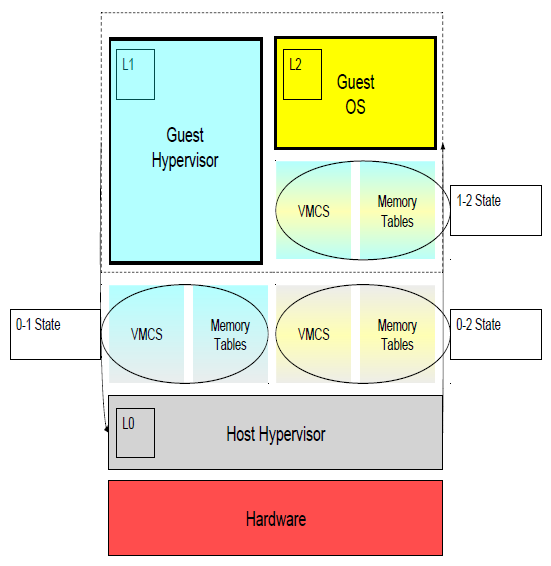
\includegraphics[width=0.7\textwidth]{chap3/nested.png}
  \bicaption[fig:nested]{嵌套式虚拟化示意图}{嵌套式虚拟化示意图}{Fig}{Illustration on nested virtualization}
\end{figure}

图\ref{fig:nested}展示了典型嵌套式虚拟化平台的主体结构,其中主要包含了L0、L1和L2三个层次。

\begin{itemize}
\item{L0(Host hypervisor):嵌套式虚拟化层,处于根模式运行。L1和L2中发生VMExit后均会陷入至此。}
\item{L1(Guest hypervisor):即为原虚拟机监控器,处于非根模式运行。为L2提供运行虚拟化支撑的同时受到L0的管控。}
\item{L2(Guest VM):即为原客户虚拟机,处于非根模式运行。用户应用程序在此运行。}
\end{itemize}

x86处理器硬件上主要有两个结构对非根模式下的运行进行控制,分别是VMCS(Virtual Machine Control Structure)和EPT。嵌套式虚拟化层L0为了支撑原虚拟机监控器L1的运行,为其准备了VMCS和EPT,我们将这一部分状态定义为“0-1状态”。原虚拟机监控器L1为了支撑原客户虚拟机L2的运行,同样为其准备了VMCS和EPT,我们将这一部分状态定义为“1-2状态”。然而,x86处理器没有从硬件上直接支持多层嵌套虚拟化(只有根模式和非根模式两种运行权限级别),也就是说实际上L1和L2处在同样的权限级别均在L0的管控下直接运行,因此L0需要为L2的运行提供额外的VMCS和EPT(相当于0-1状态和1-2状态的合并),我们将其定义为“0-2状态”。下文说明了嵌套式虚拟化系统运行的一个典型流程。

\begin{enumerate}
\item L0以VMCS0-1运行L1
\item L1准备VMCS1-2并执行vmlaunch/vmresume启动L2
\item vmlaunch产生陷入至L0,执行流由L0接管
\item L0将VMCS0-1和VMCS1-2合并,生成VMCS0-2
\item L0以VMCS0-2运行L2
\item L2在非根模式下运行,一段时间后产生陷入
\item 执行流再次由L0接管,L0根据VMExit类型选择自己处理或传递给L1处理
\item 如果L0自己能处理陷入,则vmresume继续执行L2。如果必须交给L1处理,L0根据VMCS0-2准备VMCS0-1和VMCS1-2,并将执行流切换到L1
\item 在1\~~8或5\~~8之间重复
\end{enumerate}

\subsection{系统总体架构}





\section{对客户虚拟机内存的安全保护}



\subsection{基本原理}

\subsection{特殊边界情形处理}




\section{对客户虚拟机磁盘数据的安全保护}

\subsection{基本原理}

在正常的磁盘虚拟化过程中,磁盘读取即是虚拟机监控器将被请求的磁盘数据块从磁盘映像中取出并放置到客户虚拟机指定的内存位置。反之,磁盘写入则是虚拟机监控器从客户虚拟机指定内存位置获取待写数据并存储到磁盘映像相应位置。

由于L2客户虚拟机的设备IO部分仍由L1虚拟机监控器来模拟,L1负责L2实际磁盘IO数据的读取和保存,L2的RAW磁盘映像亦被存储在L1,完全绕过L1不让其接触L2的磁盘IO数据是不实际的。而我们又要保护L2磁盘IO的安全性,故只能退而求其次,让L1始终只能接触到L2加密后的磁盘IO数据。在加密密钥没有被泄露给L1的前提下,加过密的磁盘IO数据对于L1是没有意义的。

要做到这一点,以下四个条件必须得到满足:

\begin{itemize}
\item{L1中存储的L2客户虚拟机磁盘映像必须事先经过加密。否则,L1可以直接以静态方式挂载访问L2磁盘分区和文件系统中的内容。}
\item{当L2进行磁盘读取时,加密后的L2磁盘数据必须要在L1将其读取到相应L2内存空间之后和L2实际使用这一部分数据之前,得到解密。且解密后的这部分数据存在的L2内存空间,L1是被禁止访问的。}
\item{当L2进行磁盘写入时,原先的明文L2待写磁盘数据必须要在L1能接触到其并将其写入磁盘映像之前,得到加密。也就是说,待写磁盘数据在被加密前,其所存在的L2内存空间,L1是被禁止访问的。}
\item{以上三个条件必须做到对L2完全透明,对L1基本透明(L1其实可以发现其上保存的L2磁盘映像是经过加密的)。}
\end{itemize}

对于第一个条件,我们可以用现有的成熟加解密方案处理L2磁盘映像,如AES和DES。

对于第二和第三个条件,L0可以为之完成相应的加解密工作,也可以限制L1对L2的访存范围(通过上节论述)。这里隐含的一个条件是,L0必须能够及时地获取执行机会,也就是说,在需要L0进行加解密时L0必须要得到及时通知。万幸的是,L2客户虚拟机在进行磁盘读取和写入时,均包含了一些敏感操作(IO指令或读写MMIO地址),会立即产生到L0的虚拟机陷入(VMExit),从而让L0得到通知。

对于第四个条件,L2始终接触到的均是明文数据,其不会觉察到L0和L1在事关其磁盘数据安全上做出的斗争。对于L1,除了观察到磁盘映像经过加密这一事实外,在其不威胁L2磁盘数据安全的前提下,其所经历的行为也和正常磁盘虚拟化过程无二致。


\subsection{PIO读部分的处理}

在L2客户操作系统刚启动时,其通过PIO(Programmed Input/Output)的方式读取磁盘数据。PIO是一种同步的简单磁盘数据访问方式。x86处理器上有256个IO端口,其中的一部分被预留给了IDE控制器,如下表所示。而处理器通过x86 ISA中的IO指令(in、out、ins、outs)来读写这些IO端口,来达到访问磁盘数据的目的。PIO的过程是同步的,处理器在执行这些IO指令时不能进行其他工作。

\begin{table}[!htpb]
\bicaption[tab:pio]{磁盘PIO对IO端口的使用说明表}{磁盘PIO对IO端口的使用说明表}{Table}{x86 IO port used in disk PIO}
\centering
\resizebox{\textwidth}{!}{
\begin{tabular}{ccc}
\toprule
Port Offset	& Function & Description\\
\midrule
0	& Data Port	& Read/Write PIO data bytes on this port.\\
1	& Features / Error Information	& Usually used for ATAPI devices.\\
2	& Sector Count	& Number of sectors to read/write (0 is a special value).\\
3	& Sector Number / LBAlo	& This is CHS / LBA28 / LBA48 specific.\\
4	& Cylinder Low / LBAmid	& Partial Disk Sector address.\\
5	& Cylinder High / LBAhi	& Partial Disk Sector address.\\
6	& Drive / Head Port	& Used to select a drive and/or head. May supports extra address/flag bits.\\
7	& Command port / Regular Status port	& Used to send commands or read the current status.\\
\bottomrule
\end{tabular}
}
\end{table}

以下是一个典型的DMA读数据过程


\subsection{DMA读部分的处理}

\subsection{DMA写部分的处理}

\subsection{多层内存地址转换的处理}

\subsection{缺失内存地址转换的处理}

\subsection{加解密方案与数据完整性保护}







\section{实验与性能测试}



\section{相关研究工作分析}



\section{本章小结}
